\documentclass[a4paper, 12pt]{article}
\usepackage{amssymb}
\usepackage[english,italian]{babel}
\usepackage{xspace}
\usepackage{tikz}
\usepackage[newitem,newenum,neverdecrease]{paralist}
\usepackage{amsmath,amssymb,amsfonts,mathrsfs,latexsym,stmaryrd}
\usepackage{mathtools}
\usepackage{amsthm}
\usepackage{ifpdf}
\usepackage{cases}
\usepackage{listings}
\usepackage{bm}
\usepackage{titlesec}
\usepackage[T1]{fontenc}
\usepackage[utf8]{inputenc}
\usepackage{xcolor}
\usepackage{colortbl}
\usepackage{makecell}
\usepackage{geometry}
\usepackage{layout}
\usepackage{eurosym}
\usepackage{wrapfig}
\usepackage{hyperref}

\begin{document}
	
	% interlinea 1
	\linespread{1}
	
	% 2.5cm di margine su ogni lato
	\newgeometry{
		top=2.5cm,
		bottom=2.5cm,
		left=2.5cm,
		right=2.5cm
	}
	
	% --- COPERTINA ---
	\vspace{4cm}
	\begin{center}
		\includegraphics[width=0.65\textwidth]{Images/LogoGIP.png}\\
		{\Huge \emph{\textbf{OSMOS}}}\\
		\vspace{0.5cm}
		{\large Sottotitolo}\\
		\vspace{1cm}
		A cura di:
	\end{center}
	\newpage
	
	% indice
	\tableofcontents
	\newpage
	
	\section{Executive Summary}
	\newpage
	\section{Problema da risolvere}
	Ai giorni nostri sempre maggiore importanza viene attribuita alle fonti di energia rinnovabili. Tra queste, l'energia solare è particolarmente degna di nota in quanto inesauribile, disponibile in enormi quantità ed utilizzabile per produrre energia elettrica e termica.\\
	I dispositivi in grado di sfruttare tale risorsa sono i pannelli fotovoltaici e i pannelli solari termici. Impianti che sfruttano queste tecnologia sono diffusi in tutto il mondo e vengono installati in notevoli quantità sia da grandi imprese che da utenti privati. Sono diversi i vantaggi forniti dagli impianti fotovoltaici: oltre a ridurre l'inquinamento, non utilizzando combustibili fossili, permettono di godere di sgravi fiscali fino all'80\% sulle imposte andando a produrre autonomamente energia, non dovendo attingere dalla rete elettrica nazionale.\\\\
	Nel momento in cui si decide di installare un impianto fotovoltaico, si deve tenere presente non solo del costo della installazione effettiva ma anche di quello della manutenzione dell'apparecchio durante tutto il ciclo di vita, dato che ogni pannello fotovoltaico ha un tempo di vita nominale oltre il quale perde la capacità di produrre energia. La quasi totalità di questo costo di manutenzione è relativo alla pulizia del pannello: operazione fondamentale per preservare il corretto funzionamento dell'impianto.\\
	In assenza di adeguata pulizia non solo il pannello fotovoltaico si deteriora più rapidamente ma cala la sua efficienza energetica. La sporcizia che va a depositarsi sulla superficie riduce la quantità di radiazioni solari ricevute e di conseguenza anche la quantità di energia prodotta, compromettendo il ritorno economico, tanto che la perdita di prestazioni può arrivare al 30\% dell'energia prodotta dall'intero impianto. Inoltre, a seconda della locazione in cui sono posizionati i pannelli, questi possono richiedere manutenzione più o meno frequentemente.\\
	I fattori che influenzano il livello di pulizia di un pannello sono svariati: tra i più comuni vi sono piogge acide, polveri e smog, ma anche foglie, guano e sabbia. Nella figura di seguito si mostra un esempio di impianto particolarmente sporco:
	\begin{figure}[h]
		\centering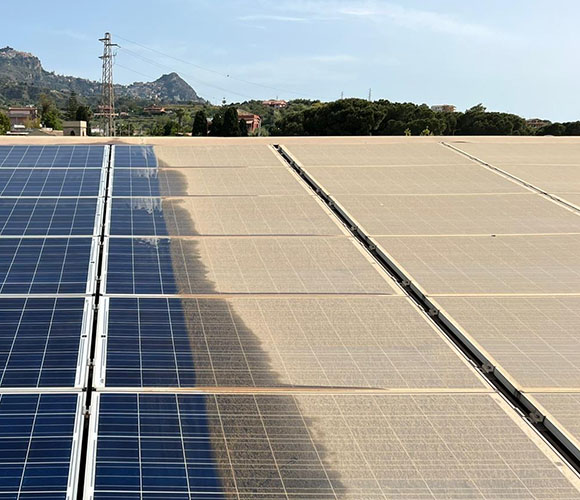
\includegraphics[width=0.5\textwidth]{Images/pannelli_sporchi2.jpg}
	\end{figure}\\
	Per affrontare il problema della pulizia, il proprietario dell'impianto può scegliere se rivolgersi ad imprese specializzate che effettuano pulizia a domicilio oppure prevenire il problema scegliendo di installare pannelli autopulenti di ultima generazione. Entrambe queste soluzioni hanno però dei limiti: per quanto riguarda la prima è l'utente stesso che deve accorgersi di quando sopraggiunge il momento opportuno per eseguire la pulizia e deve mobilitarsi per contattare l'impresa adeguata per un costo che in media varia tra i 100\euro e 300\euro.\\
	Parlando invece di pannelli autopulenti essi sono un arma a doppio taglio.\\
 Possono essere realizzati sfruttando diverse tecnologie che spaziano dall'impiego di materiali con attrito estremamente ridotto sfruttando l'acqua piovana per lavare via la sporcizia, all'uso di impulsi elettrici per far letteralmente "saltare via" le impurità dalla superficie. Tuttavia, mentre queste tecnologie di ultimissima generazione sono fuori dalla portata dei molti, l'uso di materiali dall'attrito ridotto (oltre che essere caratterizzati da costi di acquisto superiori rispetto  a pannelli tradizionali) comporta una forte dipendenza dalle precipitazioni atmosferiche che, per di più, possono anche risultare controproducenti dal momento che in aree cittadine, o generalmente più inquinate, l'acqua piovana andrebbe a depositare ulteriori detriti sulla superficie.\\
	\section{Soluzione proposta}
	La nostra proposta consiste nel fornire un sistema completamente automatizzato per la pulizia dell'impianto fotovoltaico. L'idea di base è quella di monitorare costantemente l'efficienza energetica di ogni pannello in modo tale da rendersi conto quando non è più in grado di fornire adeguate prestazioni a causa dello sporco. Quando l'efficienza scende sotto una certa soglia prestabilita dall'utente; il nostro sistema è in grado di effettuare la pulizia usando l'adeguato detergente, reso disponibile in una piccola cisterna installata nello stabile, rilasciandolo sul pannello.\\
	% immagine dell'impianto
	Questa soluzione consentirebbe al proprietario dell'impianto di risparmiare notevolmente sul costo della pulizia e sul tempo da dedicarvi, in quanto questa verrebbe effettuata automaticamente dal sistema senza che l'utente debba preoccuparsi di controllare l'impianto.\\
	Il liquido adeguato per la pulizia della superficie è l'acqua osmotica, o osmotizzata, che può assere acquistata dall'utente al costo di circa 1 \euro/L in modo che egli possa occuparsi di mantenere attivo il sistema in completa autonomia, senza dover contattare un tecnico o un'impresa specializzata.\\
	\begin{wrapfloat}{figure}{r}{0pt}
		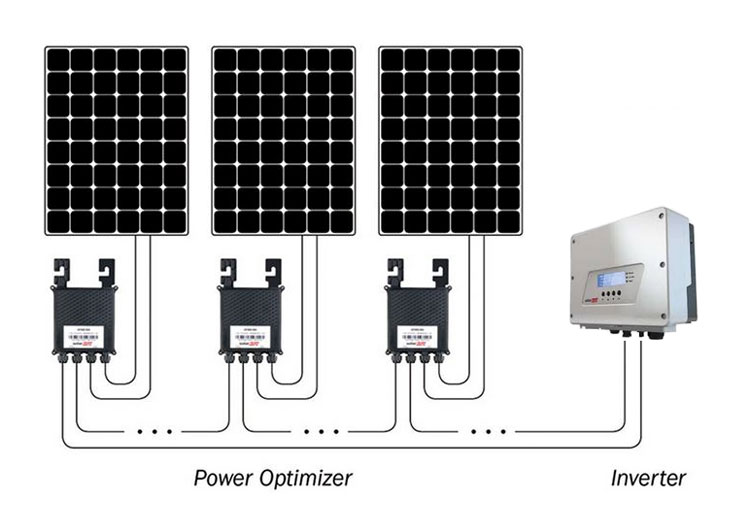
\includegraphics[width=0.5\textwidth]{Images/ottimizzatori.jpg}
	\end{wrapfloat}
	La misurazione dell'efficienza energetica è realizzabile in modo relativamente semplice. Il nostro dispositivo dialoga direttamente con gli ottimizzatori: delle componenti già presenti all'interno dell'impianto fotovoltaico, che a intervalli di tempo regolari raccolgono i report provenienti dai vari pannelli. Ciascun report contiene, tra le altre informazioni, l'efficienza energetica che può essere intercettata dal nostro dispositivo. Questo metodo di misurazione è efficace poiché, invece di sfruttare l'energia prodotta (che può variare a seconda delle condizioni atmosferiche) si basa sull'efficienza, che esprime il rapporto tra l'energia generata e l'energia solare ricevuta. Qualora il valore dovesse diminuire significherebbe che le prestazioni del pannello stanno calando e il sistema si occuperà di rilasciare il detergente sulla superficie.
	\section{Il settore}
	% https://sonnen.it/crescita-del-fotovoltaico-2023-il-boom-e-reale/ --> ho preso tanto da qua
	% https://www.lumi4innovation.it/accumulo-energia-rinnovabili-energy-storage/
	\emph{Osmos} vuole inserirsi all'interno del settore fotovoltaico, avendo lo scopo di rendere più utili e performanti queste fonti sostenibili.\\\\
	Grazie alla sempre maggiore spinta internazionale verso le fonti di energia rinnovabili, il settore fotovoltaico è in notevole espansione nel mondo.\\
	Importante è anche la crescita della capacità fotovoltaica installata in Italia. Nei primi sette mesi del 2023, in Italia, sono stati installati oltre 2,7 GW, con una crescita del 113\% rispetto allo stesso periodo dell'anno precedente e con un importante contributo degli impianti residenziali (circa il 47\% della capacità totale connessa).\\\\
	Secondo i dati forniti da \href{https://www.terna.it/it/sistema-elettrico/dispacciamento/fonti-rinnovabili}{\emph{Gaudì}}, la potenza fotovoltaica cumulata in Italia, ad agosto 2023, ha superato i 28 GW con oltre 1,4 milioni di installazioni attive. Un dato notevole se si considera che nei primi otto mesi dell'anno sono stati installati 3.123 MW di potenza fotovoltaica con andamenti diversi per i vari segmenti:
	\begin{itemize}
		\item residenziali registrati l'installazione di 1.379 MW (impianti sotto i 12 kW);
		\item commerciale ed industriale  registrati 1.088 MW (impianti tra i 20 kW e 1 MW); 
		\item utility-scale aumento di 426 MW (impianti con potenza superiore a 1 MW);
	\end{itemize}
	I dati registrati dal settore del fotovoltaico e le previsioni di crescita mostrate nelle figure di seguito, sottolineano il ruolo centrale delle fonti rinnovabili nel percorso di transizione energetica globale, riportando un indice CAGR che si aggira intorno al 30\%.
	\begin{center}
		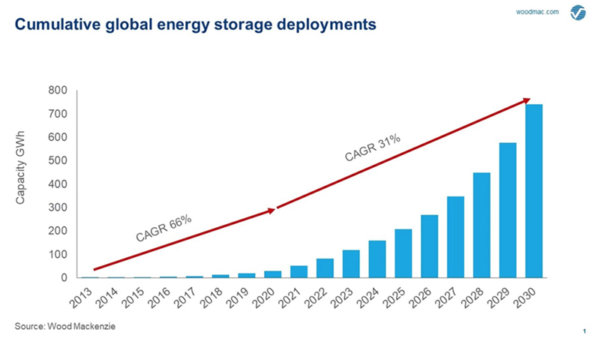
\includegraphics[width=0.9\textwidth]{Images/previsioni_solare.jpg}
		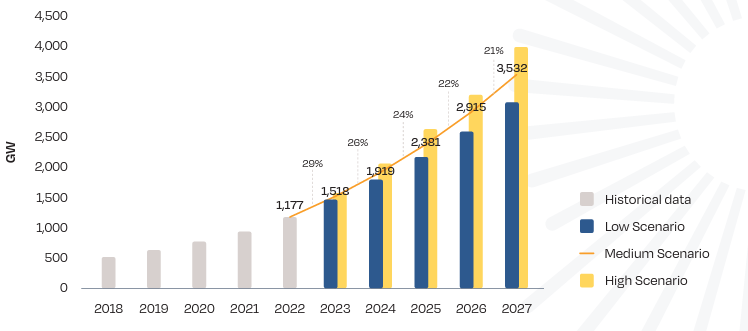
\includegraphics[width=0.73\textwidth]{Images/andamento_pannelli2.png}
	\end{center}
	Il settore del fotovoltaico è sufficientemente vasto da poter essere a sua volta suddiviso in due parti: una prima parte che comprende le imprese produttrici di moduli fotovoltaici (in cui i principali attori sono \emph{Sunpower, Panasonic, Exe Solar} e simili) e una seconda parte che riguarda le imprese produttrici di componenti cooperanti coi moduli fotovoltaici.\\\\
	Sebbene esistano enti che si pongono a cavallo di questa partizione, \emph{Osmos} fa capo solamente alla seconda categoria. All'interno di questa non vi è grande frammentazione, infatti la maggioranza è occupata da \emph{Abb Spa}: una società fortemente coinvolta nella produzione di apparecchiature che garantiscono continuità di servizio, affidabilità e ritorno dell'investimento tramite interruttori, dispositivi di misurazione, sensori e altro.\\
	I prodotti e servizi forniti da \emph{Abb Spa} sono poi utilizzabili anche in moltissimi altri settori eterogenei; questo aumenta considerevolmente l'influenza e il potere economico dell'impresa stessa, dandole la possibilità di imporsi nei confronti di altre società più specializzate quali \emph{Enel X} e \emph{SoralEdge Tecnology} come riportato nel grafico seguente:\\
	\begin{center}
		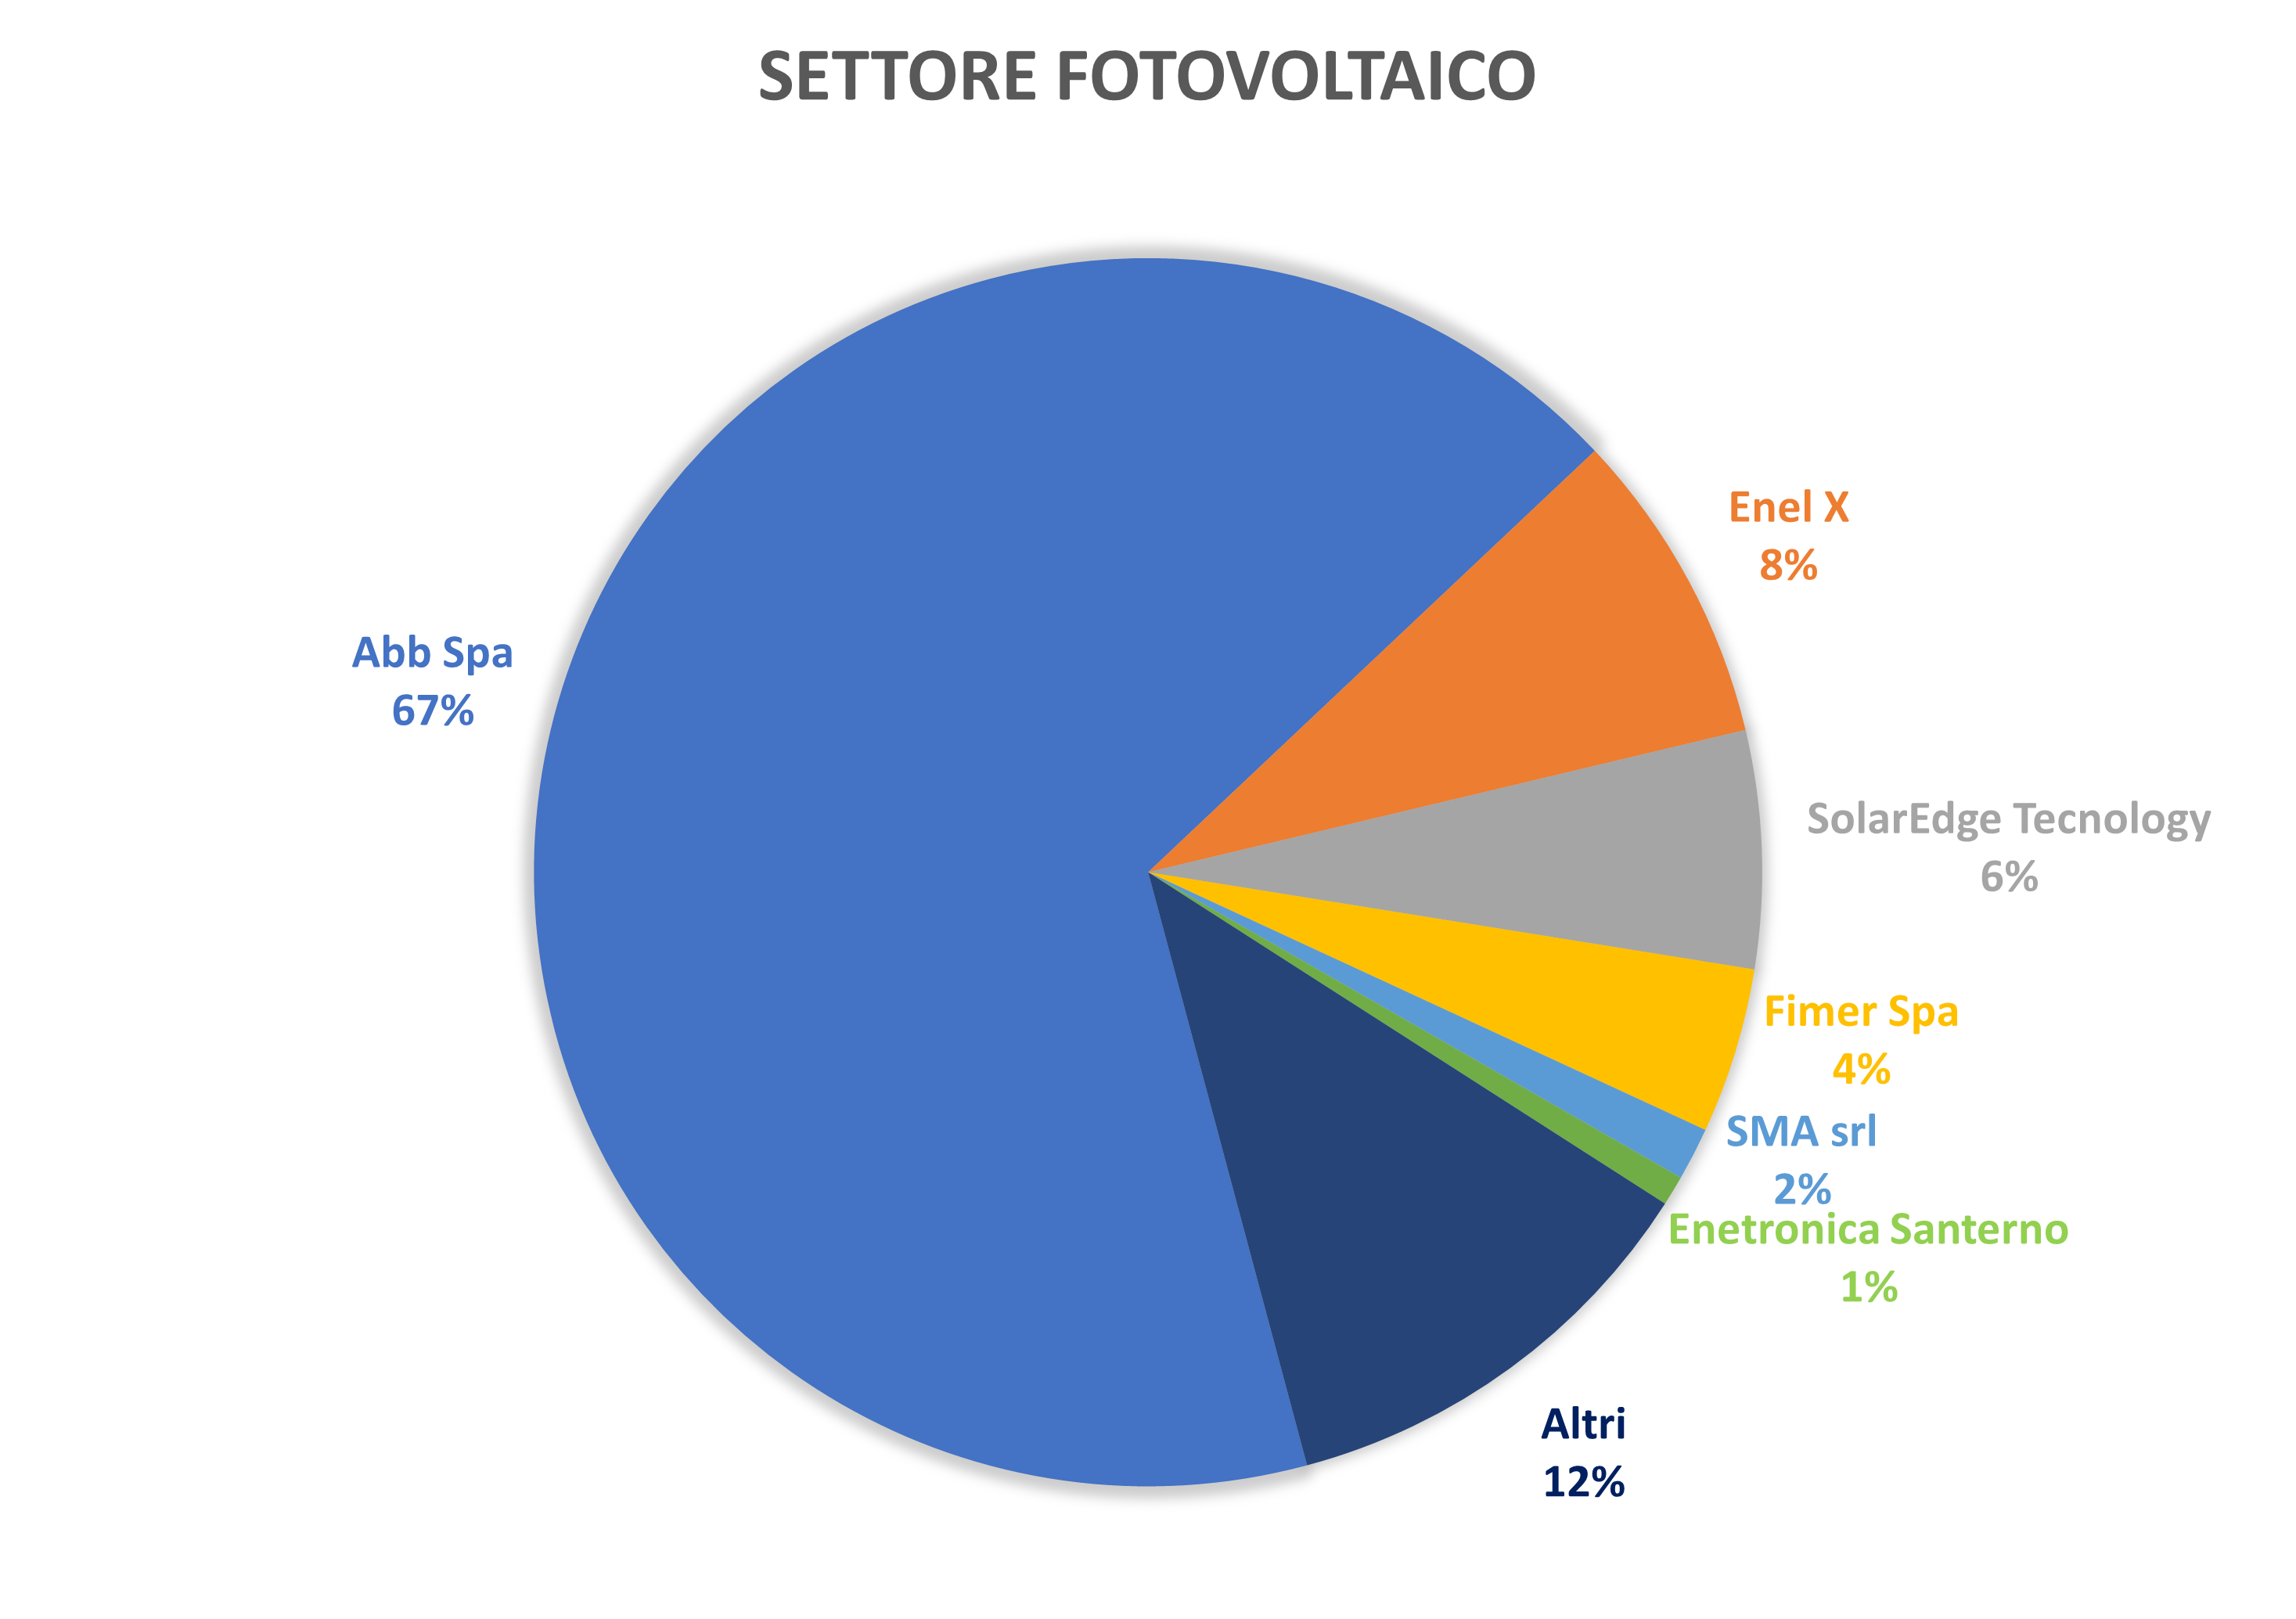
\includegraphics[width=0.7\textwidth]{Images/suddivisione_settore.png}
	\end{center}
	La proposta di \emph{Osmos} è ritenuta interessante per l'attuale situazione del settore, sia perché l'ambito del fotovoltaico si sta ampliando sia a causa della mancanza di una soluzione a supporto dei moduli fotovoltaici specializzata nella pulizia di questi.\\
	La strategia adottata è riportata di seguito:
	\begin{center}
		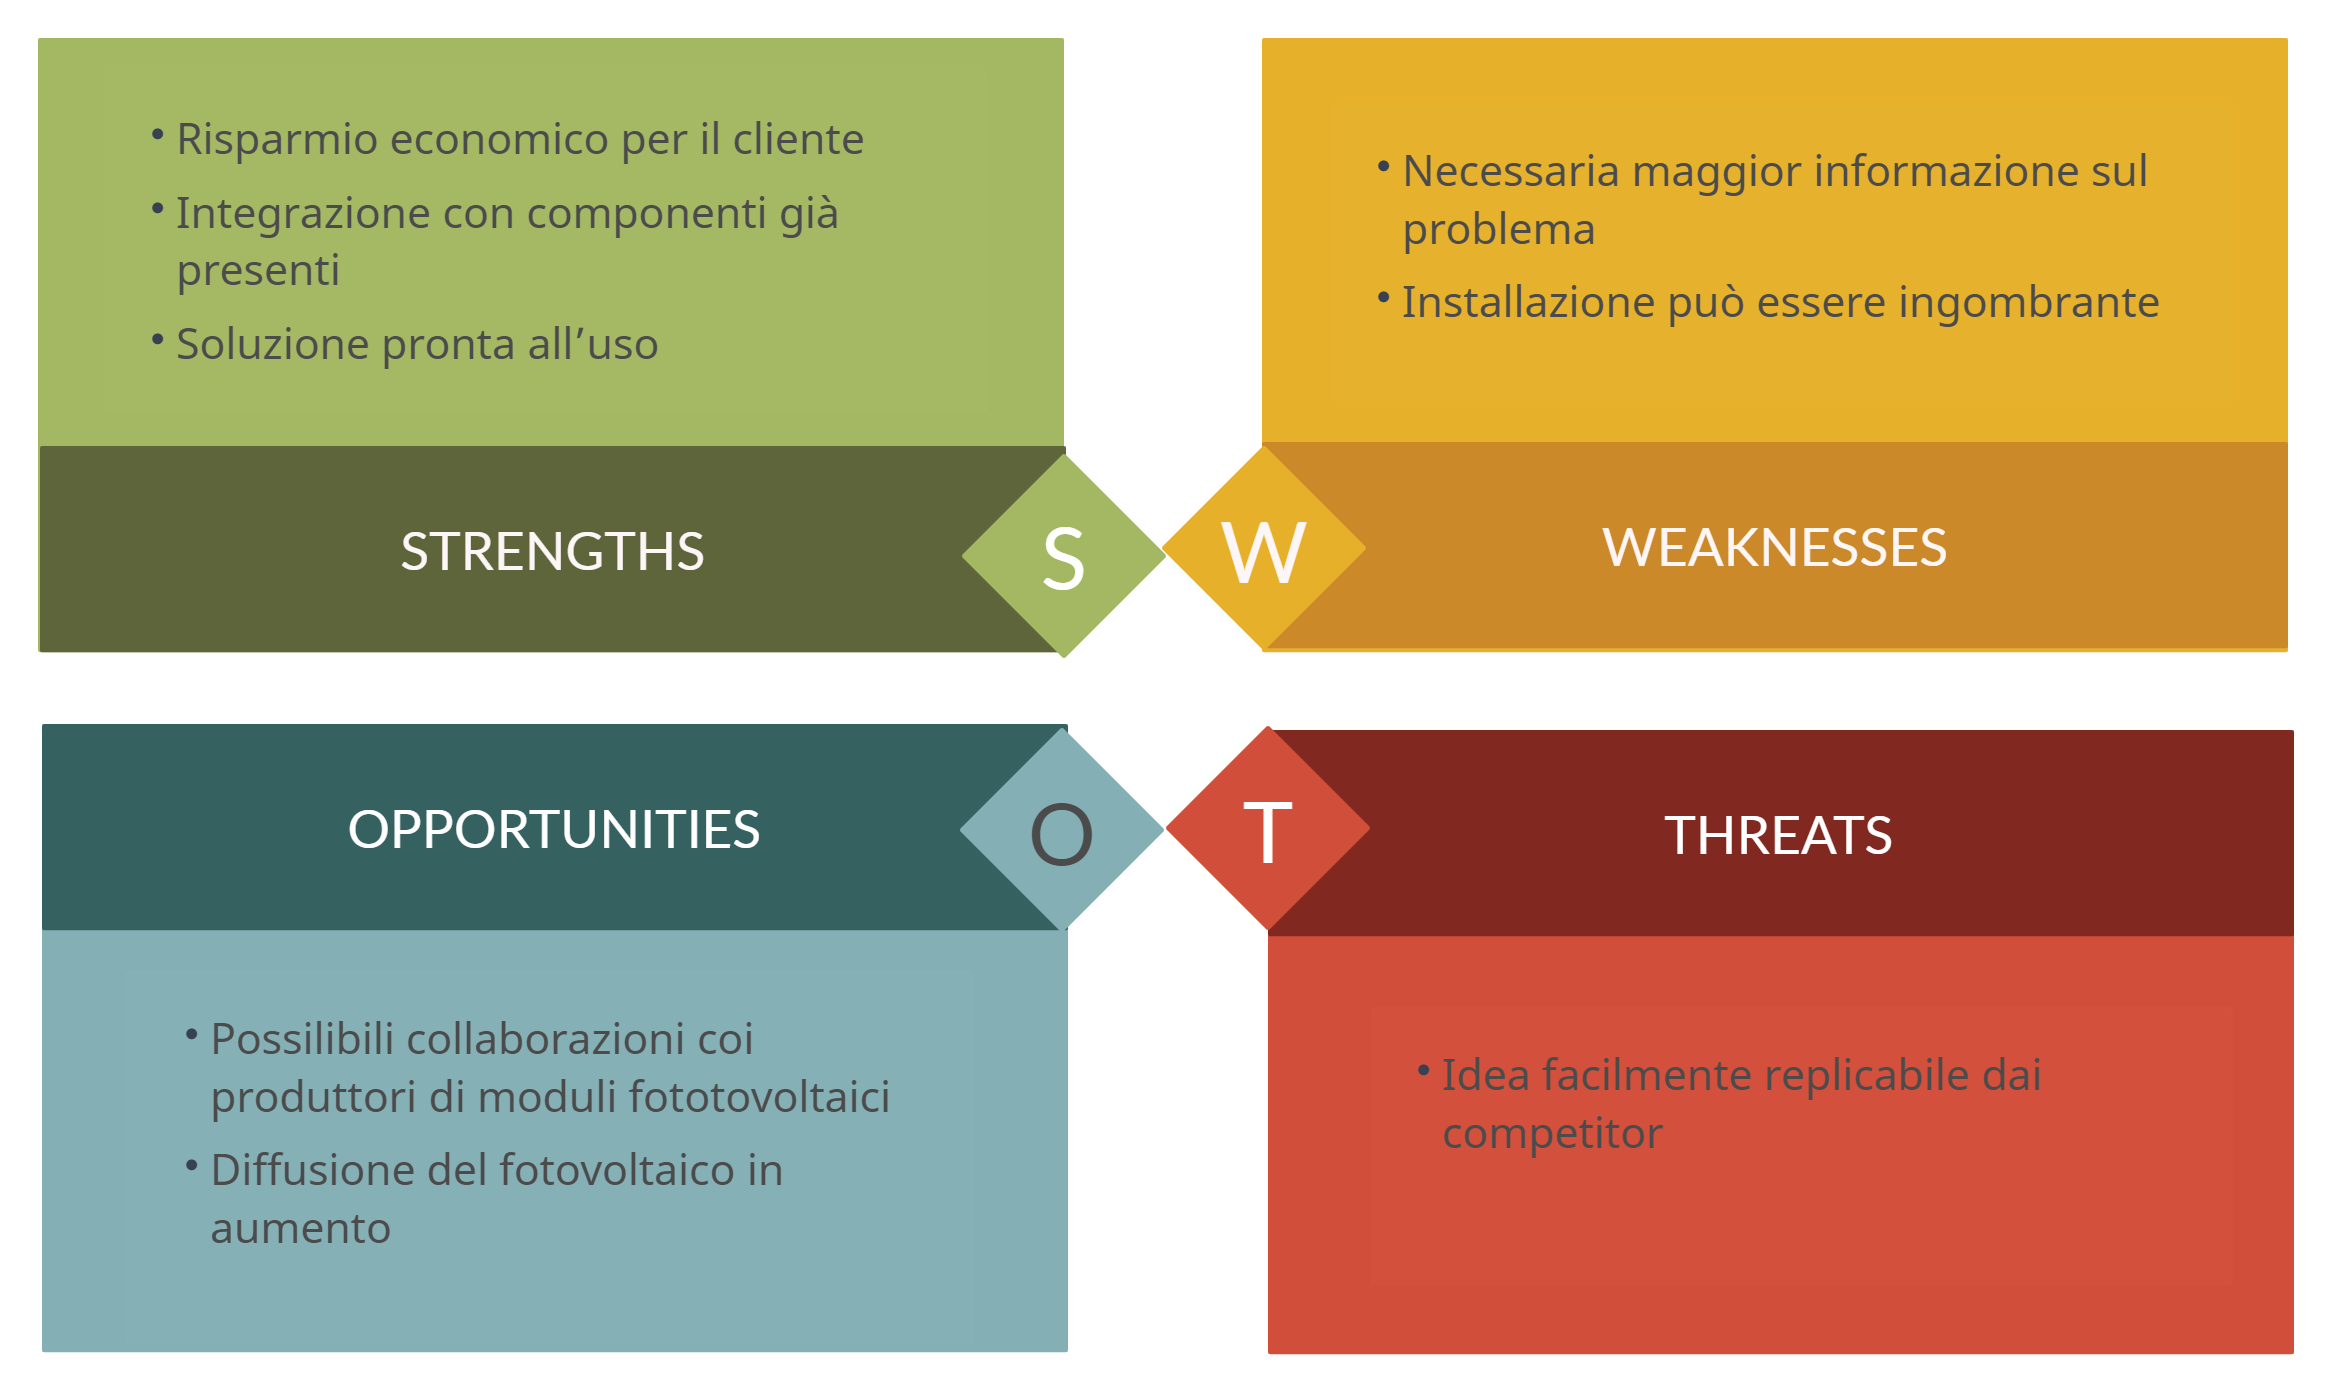
\includegraphics[width=0.65\textwidth]{Images/SWOT2.png}%\vspace{-2cm}
	\end{center}
	Inoltre si riportano qui gli obiettivi perseguiti da \emph{Osmos} confrontati con quelli dei principali competitor sopra citati:
	\begin{center}
		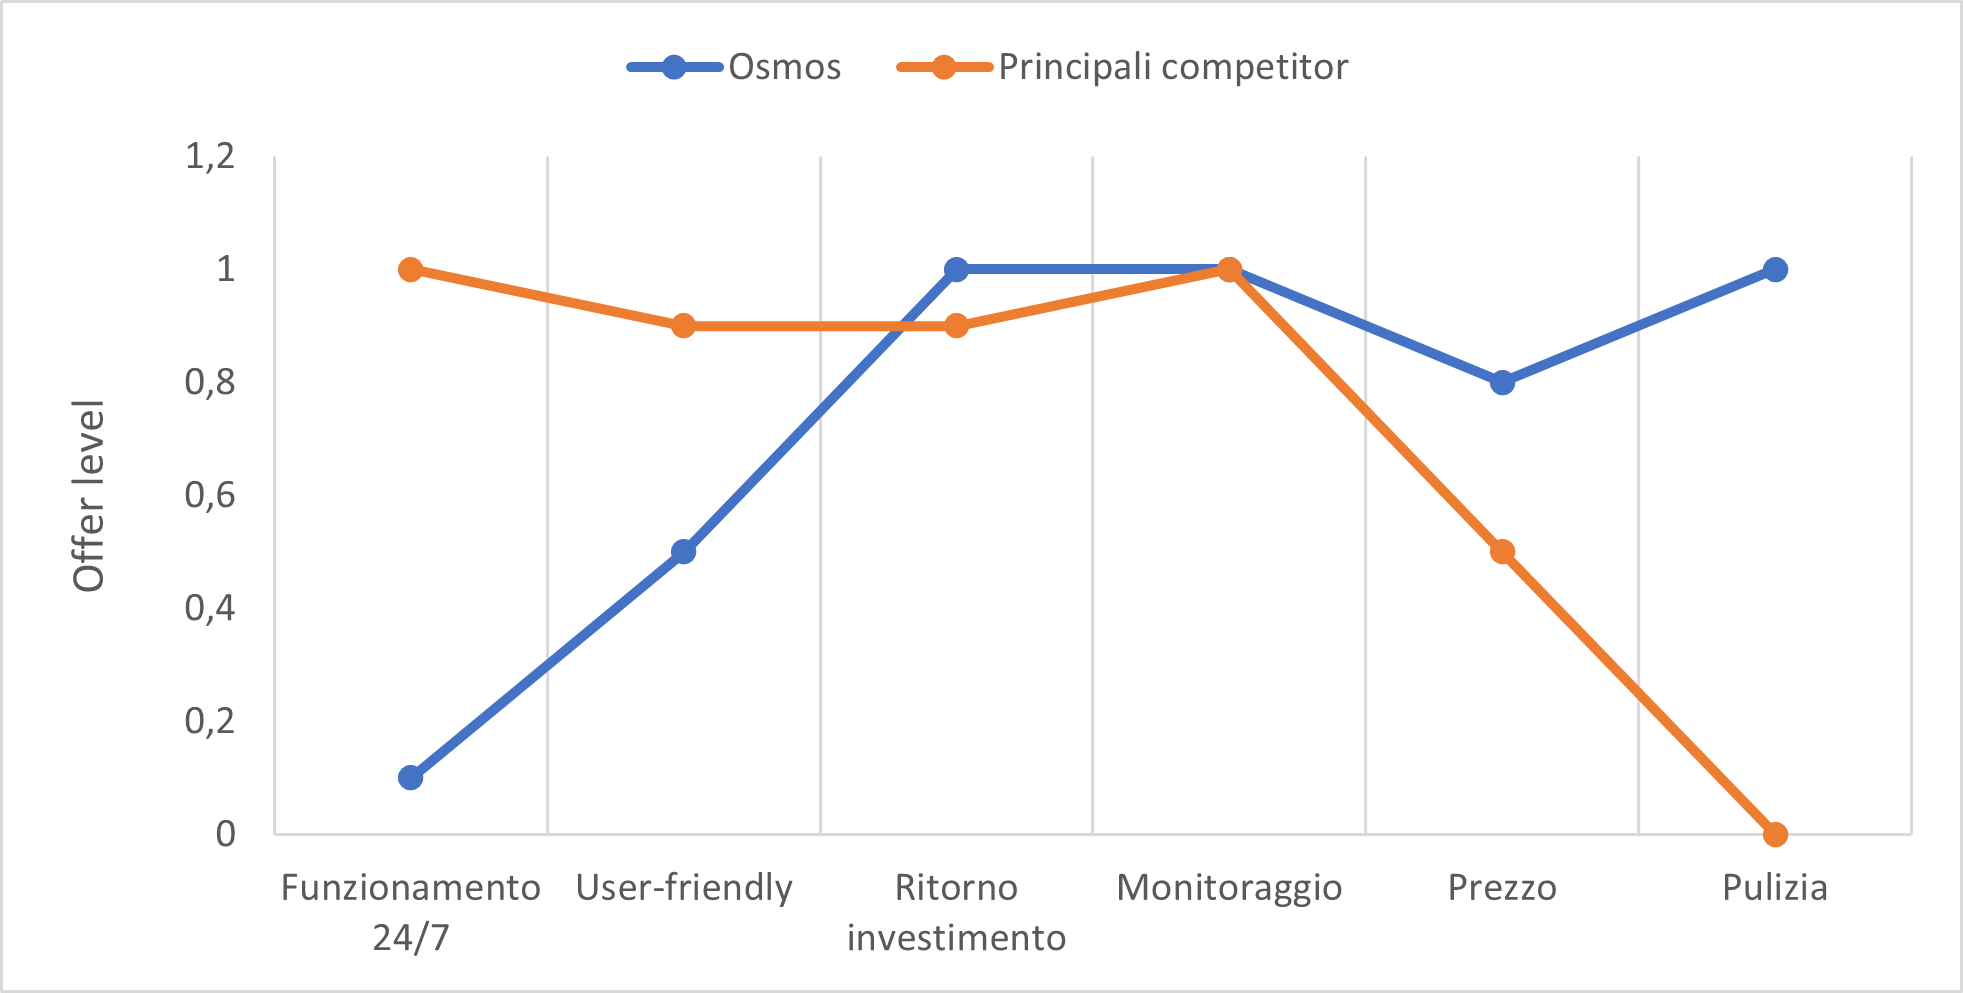
\includegraphics[width=0.8\textwidth]{Images/curve_valore.png}%\vspace{-2cm}
	\end{center}
	\section{Il mercato e il cliente}
	\begin{figure}[h]
		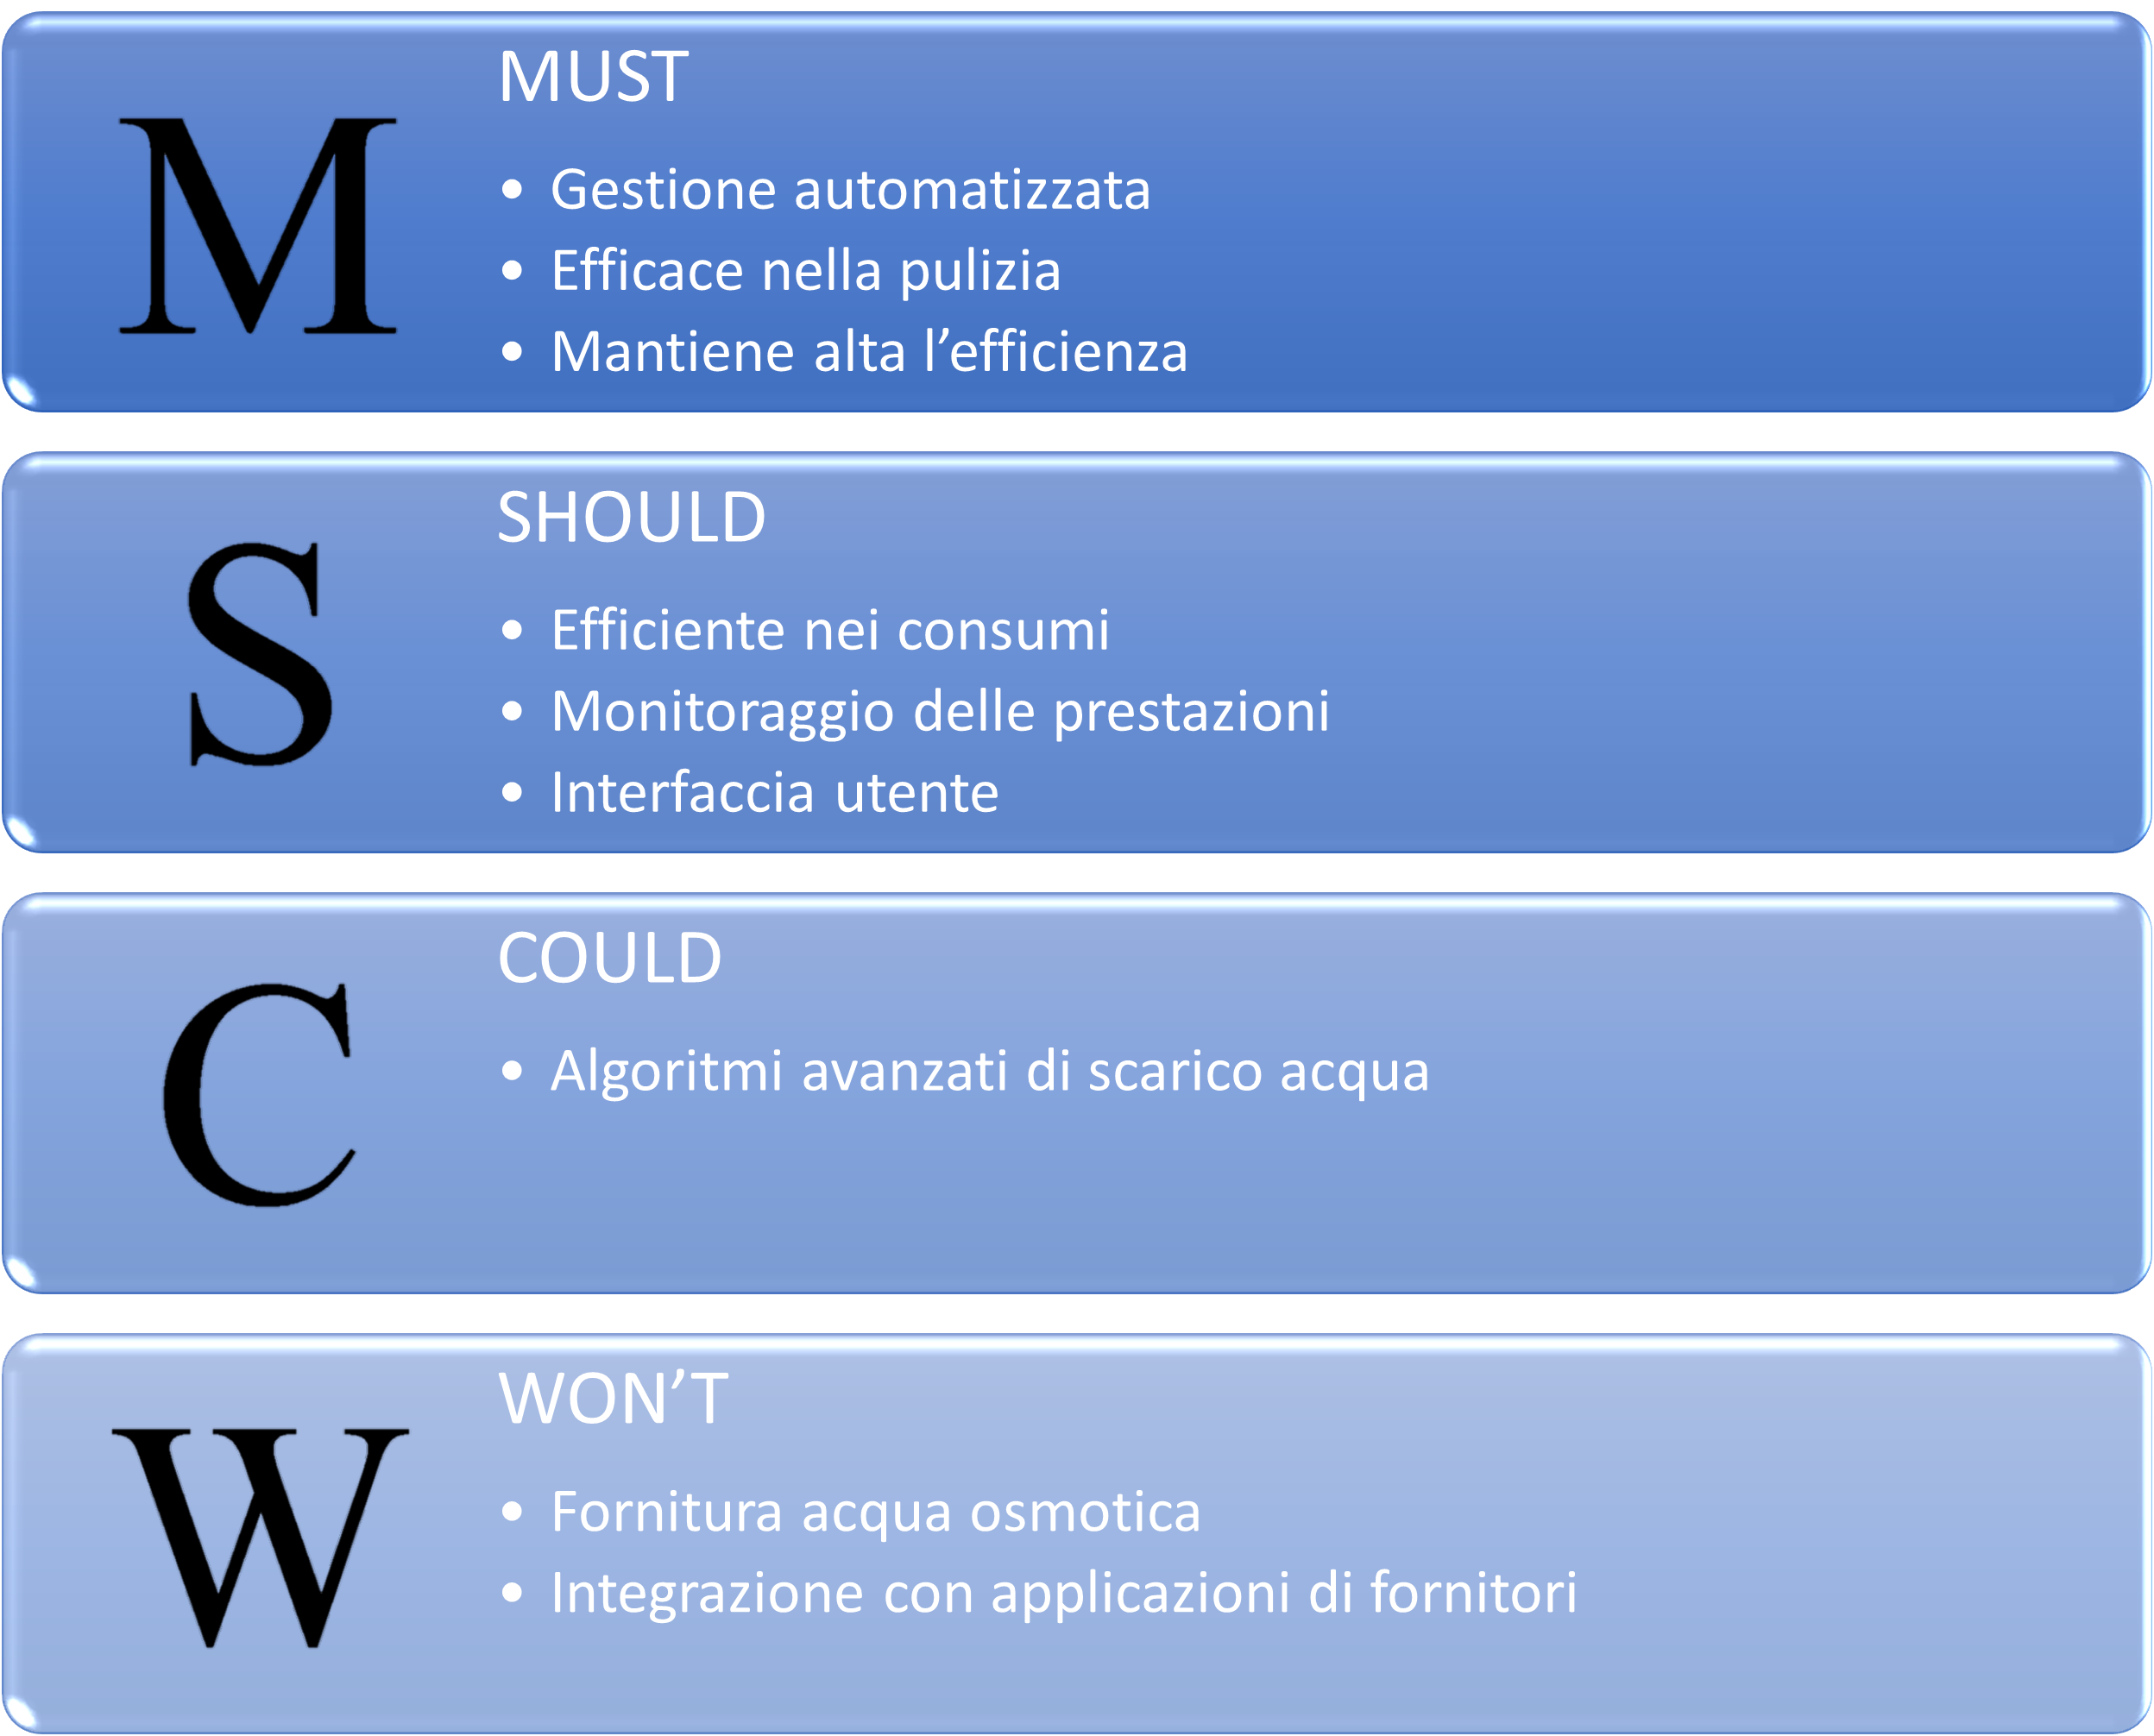
\includegraphics[width=0.5\textwidth]{Images/MoSCoW.png}
	\end{figure}
	\section{Modello di business}
	\textbf{Value Proposition}\\
	L'obiettivo di \emph{Osmos} è fornire e installare sistemi per la pulizia automatica dei moduli fotovoltaici. Questi sistemi sono indirizzati sia agli utenti privati, sia verso imprese che possiedono una superficie fotovoltaica notevolmente superiore. I sistemi proposti forniscono ai clienti non solo la possibilità di sfruttare impianti che mantengono un alto livello di efficienza energetica ma anche di risparmiare sul costo della pulizia, dal momento che non ci sarà più la necessità di rivolgersi ad una ditta esterna per eseguirla.\\
	Così facendo il cliente dovrebbe unicamente occuparsi di rifornirsi di acqua osmotica per riempire il relativo serbatoio con cui poi il sistema effettua la pulizia.\\\\
	\textbf{Relazione col cliente}\\
	Il primo contatto con il cliente può essere stabilito tramite la stessa impresa produttrice e installatrice dell'impianto fotovoltaico che informa della possibile installazione anche di un sistema \emph{Osmos}, oppure tramite spot pubblicitari online attraverso social network e pubblicità mirata. In questo modo diventa possibile intercettare consumatori entranti nel settore sempre crescente del fotovoltaico, rendendoli consci del problema fin dal momento dell'acquisto dei pannelli.\\
	Una volta entrati in contatto con l'acquirente, dopo l'avvenuta installazione si ha l'obiettivo di mantenere il rapporto col cliente tramite la fornitura di un servizio di assistenza disponibile per via telefonica, utilizzabile dall'utente per contattare l'assistenza in caso di malfunzionamenti del sistema o problemi di qualsiasi genere legati ad esso, di modo da poter intervenire tempestivamente.\\\\
	\textbf{Elementi chiave}\\
	\emph{Osmos} attribuisce molto peso all'esecuzione di un sopralluogo del sito di installazione per essere in grado di pianificare la soluzione che meglio si adatta al singolo cliente.\\
	Una volta avvenuta l'installazione risulta di vitale importanza un adeguato monitoraggio dell'efficienza energetica nel tempo, reso possibile dalla storyline dell'impianto fotovoltaico. Questa garantisce l'avvio della pulizia nel momento ideale allo scopo di attestare le prestazioni su valori elevati e di prolungare la vita del modulo fotovoltaico.\\
	Notevole importanza è poi attribuita anche ai partner. Come visto in precedenza, si ha intenzione di stabilire collaborazioni con imprese fornitrici di impianti fotovoltaici. Questo garantirebbe non solo una più facile sensibilizzazione degli utenti sull'importanza della pulizia dei pannelli, ma andrebbe anche ad aumentare il bacino d'utenza del settore.\\ % si capisco il senso dell'ultima frase? si / fa un po schif, l'ho riarrangiata (matte)
	Inoltre, avendo la possibilità di stipulare contratti con le imprese fornitrici di materie prime (quali componenti elettroniche e componenti idrauliche) si andrebbero a ridurre i costi di produzione, aumentando di conseguenza il margine di profitto.\\\\
	% idee:
	%	- adeguata pianificazione dell'installazione nel domicilio: soluzione applicata ad hoc per il cliente (attività)
	%	- collaborazione con impresa che installa pannelli (partner chiave) grazie ad essa si facilità la divulgazione del prblema che andiamo a risolvere
	%	- forniori di materie prime sia Arduino che a livello idraulico (partner)
	\textbf{Analisi costi e ricavi}\\
	In Italia, il costo medio per effettuare una pulizia completa dell'impianto si aggira tra i 100 e i 300\euro: un costo che varia a seconda della condizione in cui versano i pannelli, della posizione n ella quale questi sono installati e dalle dimensioni della superficie. \emph{Osmos} punta a fornire un prodotto dal costo complessivo e indicativo per il cliente finale di 500\euro: un prezzo dato in gran parte dalla manodopera in fase di installazione ma variabile proprio in base a questa.\\
	Il costo delle materie prime è invece più limitato: oltre al software necessario (di nostra produzione) è richiesto solamente un modulo Arduino e le componenti idrauliche, per un costo totale stimato di 120\euro.\\
	L'obiettivo risulta quello di ottenere un profitto del 20\% su ogni installazione.
	% sopra hai parlato di un servizio di manutenzione, qua non sarebbe da includere? è ad abbonamento?
	\begin{center}
		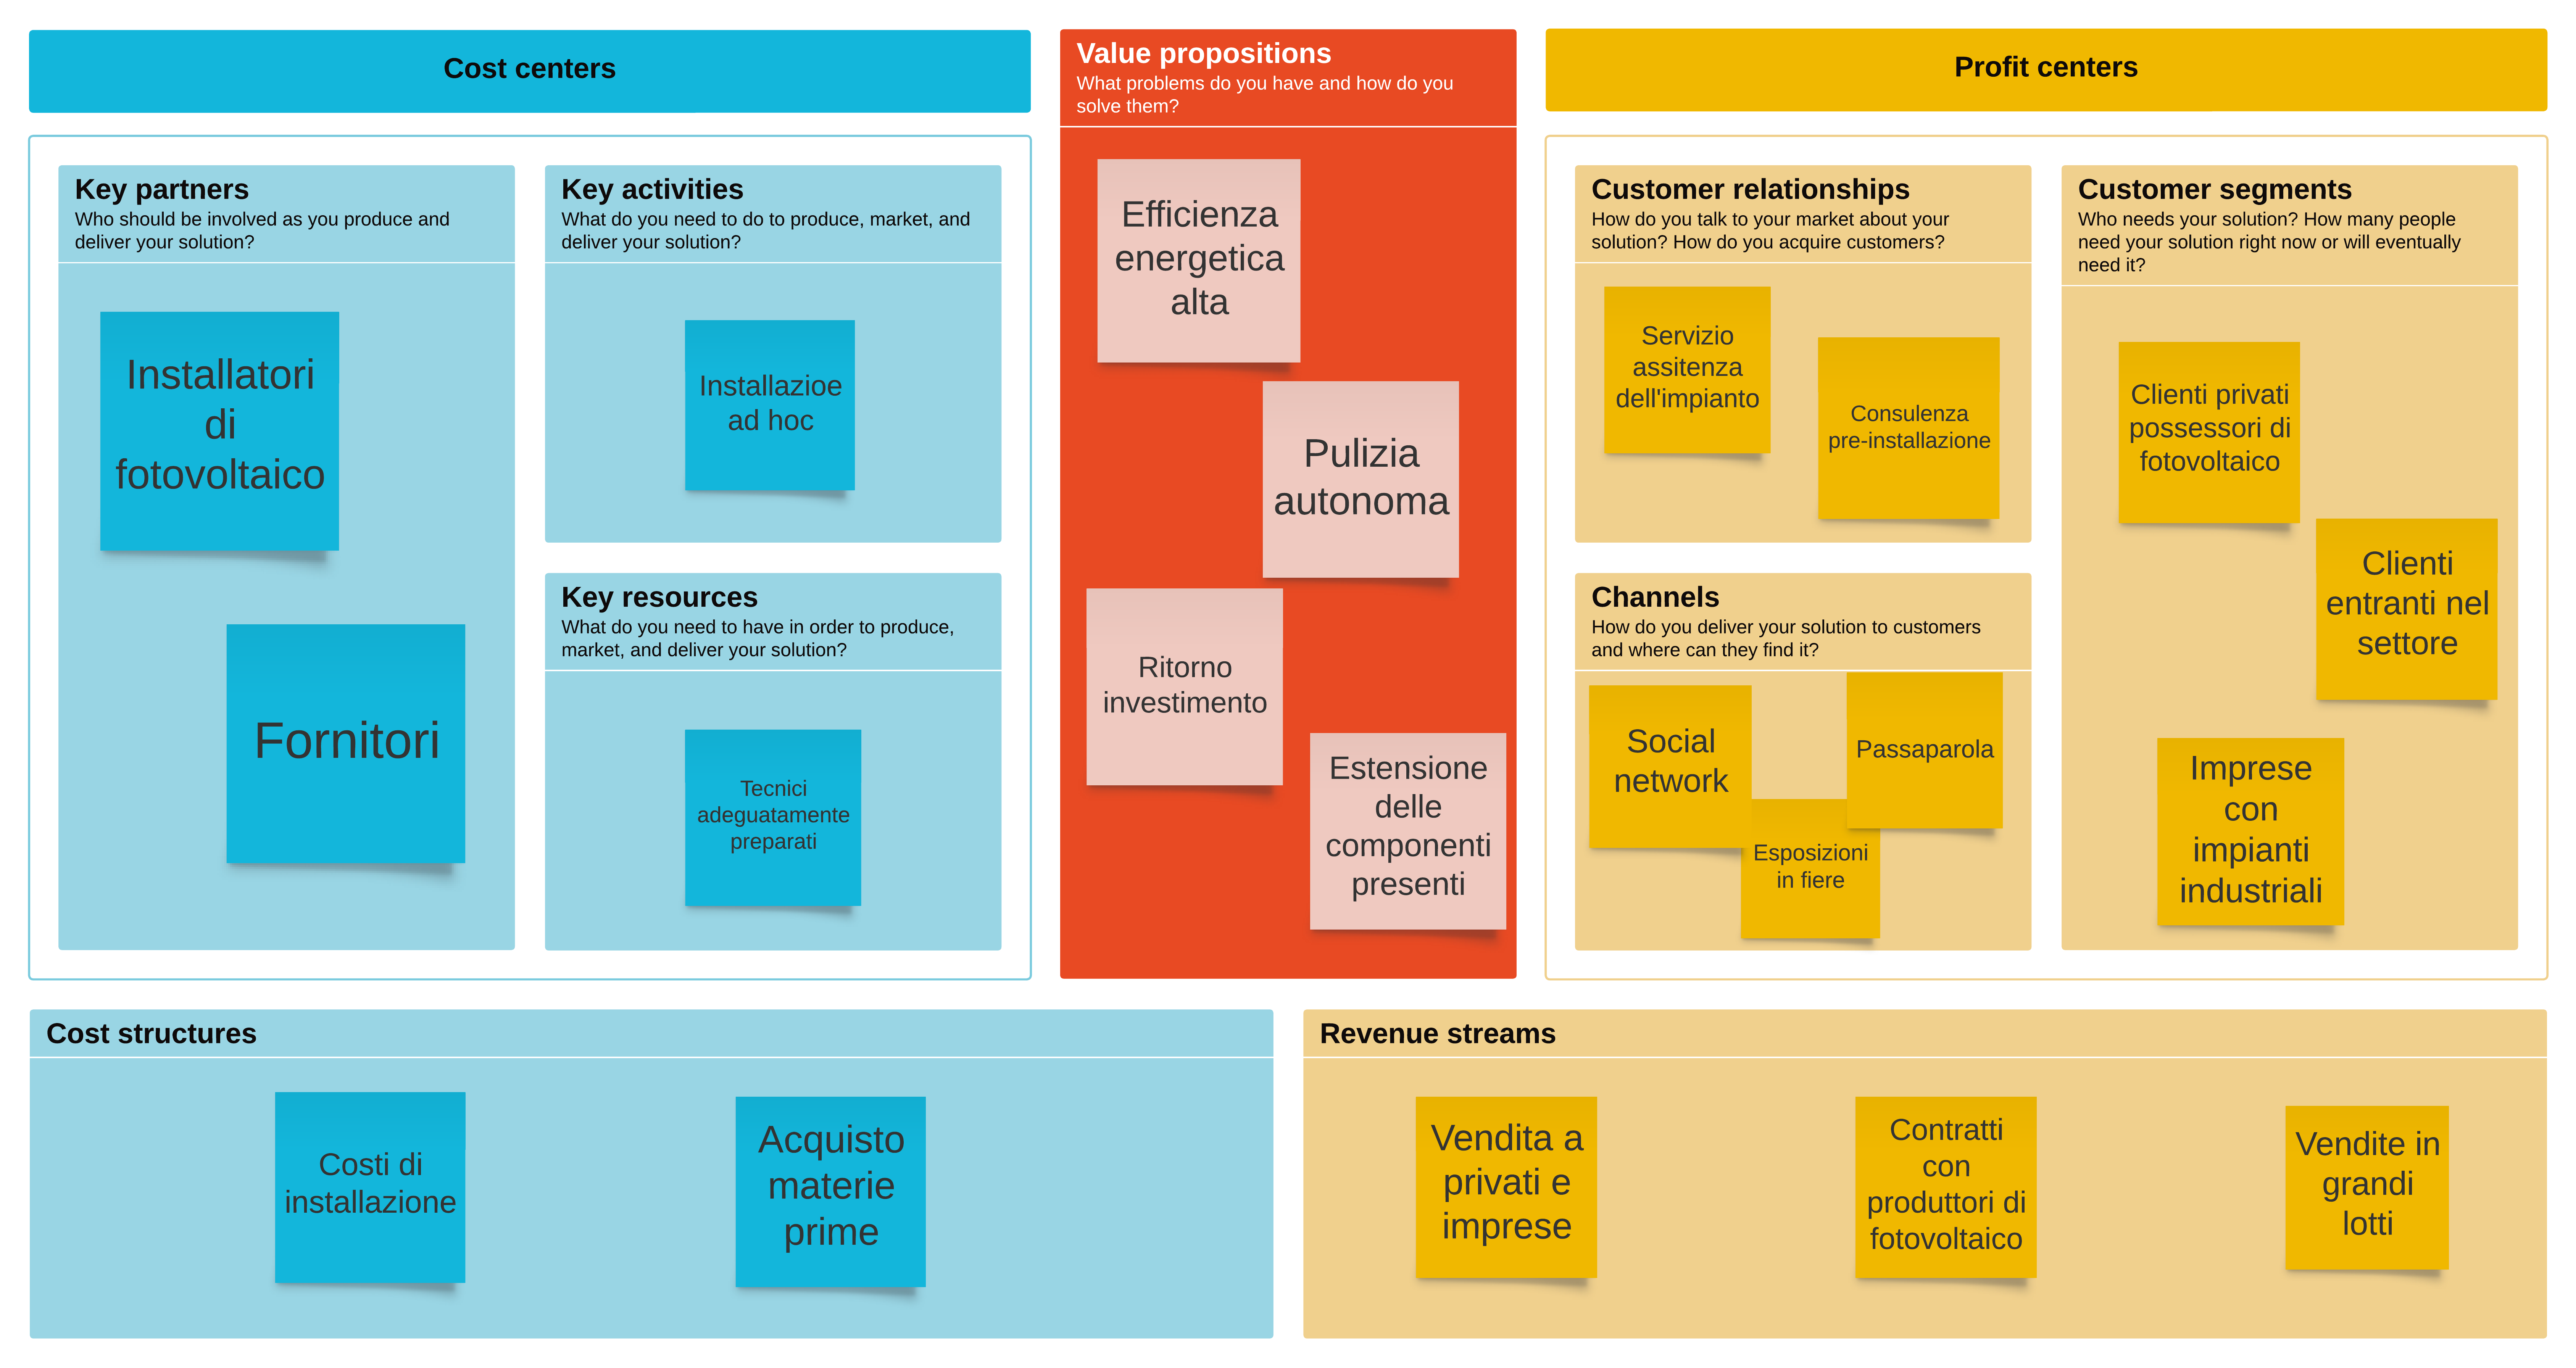
\includegraphics[width=0.9\textwidth]{Images/BusinessModelCanvas.png}
	\end{center}
	% idee:
	%	- esprimere il costo di una tradizionale pulizia, il nostro prodotto avrà un costo circa pari a quello della singola pulizia ma consentirà al cliente di non pacgare più per altri interventi
	%	- costi: manodopera per installazione (dipende da installazione a installazione) e materie prime... diciamo un 50 euro + manodopera?
	%	- prezzo di vendita = costi + 25%?
	\section{Funzionamento del prodotto}
	

	%cosa dire:
	% descrizione introduttiva delle funzionalita offerte dalla soluzione 
	\emph{Osmos} è un sistema di supporto alla pulizia di un impianto fotovoltaico,
	 esso e composto da un device in grado di monitorare l'efficienza dei pannelli 
	 e un supporto idraulico per il rilascio del detergente sul pannello.\\Di seguito un immagine del prodotto


	\begin{center}
		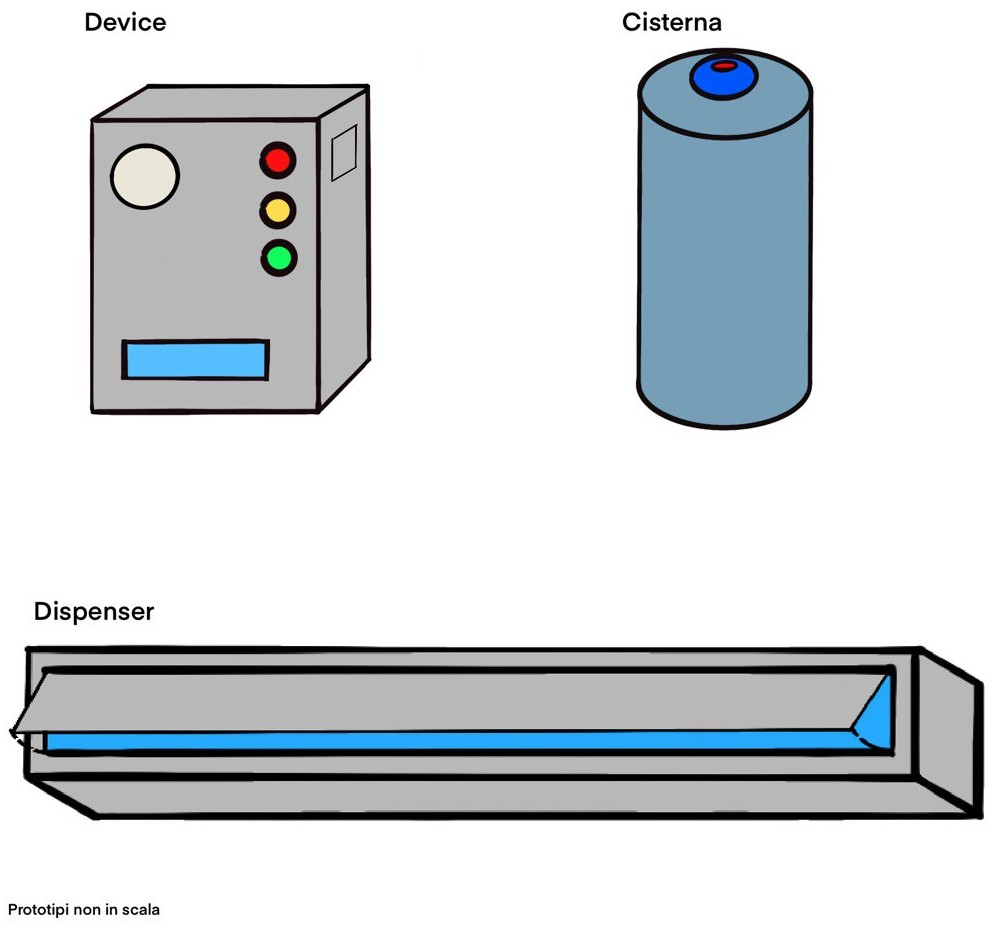
\includegraphics[width=0.5\textwidth]{Images/prototipo.jpg}
	\end{center}

	% descrizione del device principale
	Il device principale si compone di un microcontrollore in grado di monitorare l'efficienza energetica dei pannelli.
	Cio viene fatto intercettando tramite rete wireless i report prodotti dagli ottimizzatori installati nell'impianto fotovoltaico
	le informazioni raccolte vengono mantenute all' interno del sistema in modo da mantenere uno storico dello stato recente dell'impanto.
	Il dispositivo dispone di un display e un interfaccia a led che mostrano l'efficienza in percentuale dell'impianto 
	Il sistema avvia la pulizia del pannello quando l'efficienza cala sotto la soglia configurabile dall' utente, 
	oppure su interazione dell'utente tramite un pulsante posto sul device.
	Quando viene avviata la procedura di pulizia il device attiva un sistema idraulico che versa l'apposito detergente sul pannello\\
	\\
	
	% descrizione del sistema idraulico
	Il supporto idraulico del sistema e composto da una pompa idraulica e un serbatoio contenente il detergente. 
	Al momento della pulizia la pompa idraulica viene attivata per scaricare tramite un apposito sportello il detergente sulla superficie,
	il detergente esausto viene smaltito dal sistema nella rete idraulica dell' edificio.
	Il sistema prevede un facile accesso al serbatoio in modo da facilitare le operazioni di carico del detergente.
	% MONSTER ALLERGY MI FAN STARNUTIR
	% quali tecnologie gia esistenti sfrutta la soluzione

	\section{WBS e prospetto di Gantt}
	In precedenza sono stati elencati gli elementi e attività fondamentali per \emph{Osmos}. Questi possono essere pianificati racchiudendoli in 4 macro attività che rappresentano l'intero progetto:
	\begin{enumerate}
		\item \textbf{Project management}\\
			  L'insieme delle attività riguardanti la pianificazione, la gestione delle risorse e lo studio dell'ambito dell'impresa tramite analisi del settore e analisi del mercato. L'output di questo \emph{work package} è un documento contenente tutti i dati necessari e ad ottimizzare il lavoro successivo, come adeguate conoscenze del segmento di mercato selezionato oppure lo schedule dei lavori successivi.
		\item \textbf{Prototipazione}\\
			  Le attività che hanno come output finale la realizzazione di un MVP specifico, da mostrare ad investitori ed \emph{early adopters} in grado di rendere l'idea di ciò che sarà il prodotto finale, implementando solo quelle caratteristiche per cui il cliente è disposto a pagare: la gestione automatica della pulizia e il monitoraggio dell'efficienza. L'MVP consentirà di testare e validare le idee del prodotto senza spreco economico e temporale nella realizzazione del prodotto completo.
		\item \textbf{Produzione}\\
			  Superate le prime fasi di vita dell'impresa, \emph{Osmos} dovrà occuparsi della vera e propria realizzazione dei prodotti completi. Questo \emph{work package} raccoglie quindi le attività di ottenimento delle materie prime e costruzione, assemblaggio vero e proprio, del prodotto finito.
		\item \textbf{Commercializzazione}\\
			  Ultimo insieme di attività che può anche essere eseguito parzialmente in parallelo col precedente. Rappresenta principalmente il rapporto col cliente.
	\end{enumerate}
	Di seguito è riportata la struttura delle WBS nel dettaglio:
	\begin{center}
		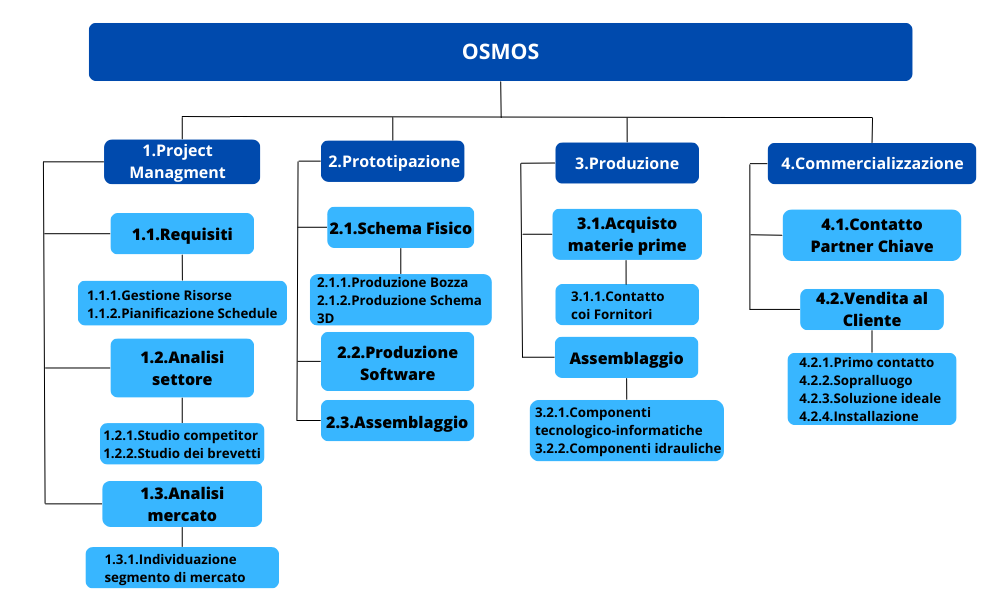
\includegraphics[width=0.9\textwidth]{Images/WBS.png}
	\end{center}
	Ad ogni singola WBS che è riportata in questa struttura gerarchica sono associati vincoli temporali per il loro completamento. Le diverse attività sono inoltre assegnati a 3 diversi team operativi:
	\begin{itemize}
		\item Team A $\rightarrow$ si occupa sia della fase di pianificazione sia della parte organizzativa legata alla gestione delle risorse materiali e non;
		\item Team B $\rightarrow$ dedicato inizialmente alla realizzazione del prototipo, successivamente avrà il compito di occuparsi dell'assemblaggio dei prodotti finiti prima della consegna al cliente;
		\item Team C $\rightarrow$ il cui compito sarà relazionarsi col cliente presentandogli il prodotto, individuando la soluzione più adatta e procedendo con l'installazione a domicilio.
	\end{itemize}
	Gli obiettivi temporali sono riportati nel seguente diagramma di Gantt. Per completezza, un diagramma maggiormente dettagliato è presente in appendice.
	\begin{center}
		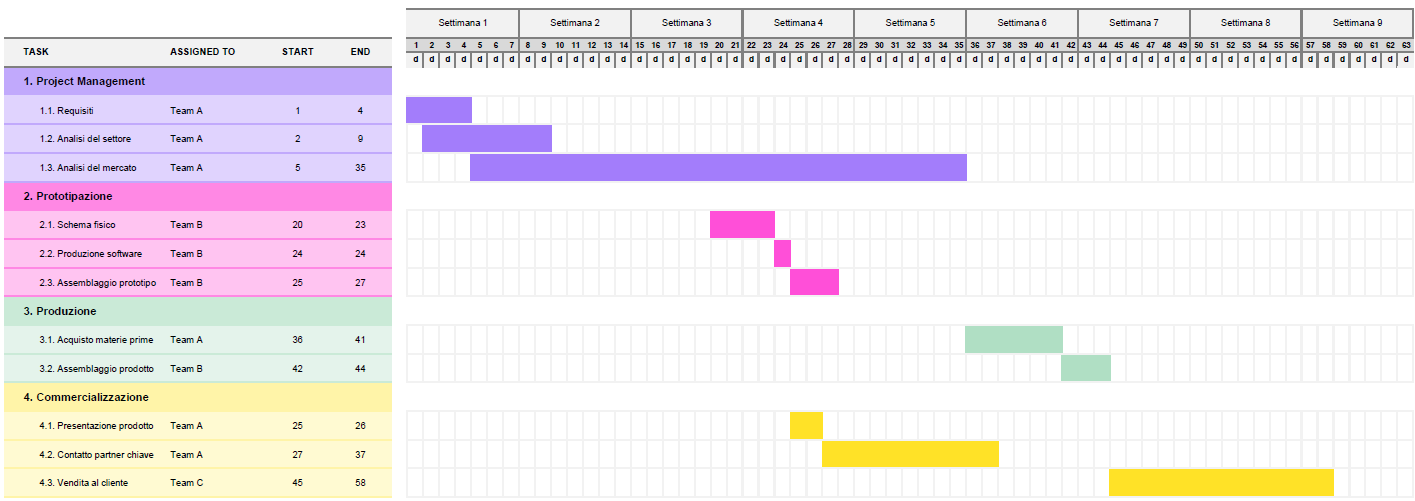
\includegraphics[width=\textwidth]{Images/gantt.png}
	\end{center}
	\newpage
	\section{Appendice}
	Elemento \#1 - Prospetto di Gantt completo
	\begin{center}
		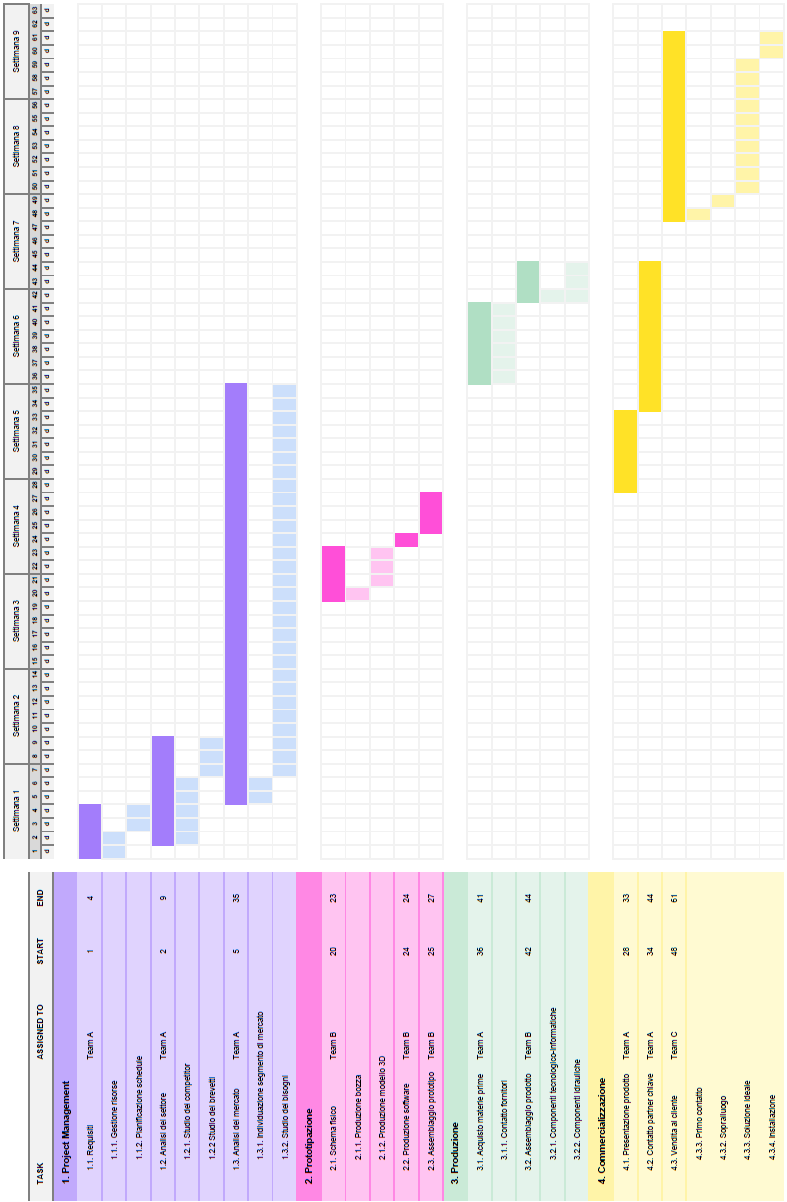
\includegraphics[width=0.9\textwidth]{Images/gantt_full.png}
	\end{center}
\end{document} 
